%\documentclass[wcp,gray]{jmlr} % test grayscale version
 %\documentclass[wcp]{jmlr}% former name JMLR W\&CP
\documentclass[pmlr]{jmlr}% new name PMLR (Proceedings of Machine Learning)

 % The following packages will be automatically loaded:
 % amsmath, amssymb, natbib, graphicx, url, algorithm2e

 %\usepackage{rotating}% for sideways figures and tables
\usepackage{longtable}% for long tables

 % The booktabs package is used by this sample document
 % (it provides \toprule, \midrule and \bottomrule).
 % 
 % book quality tables
 \usepackage{booktabs}
 
 % The siunitx package is used by this sample document
 % to align numbers in a column by their decimal point.
 % Remove the next line if you don't require it.
\usepackage[load-configurations=version-1]{siunitx} % newer version
 %\usepackage{siunitx}

\makeatletter
\def\set@curr@file#1{\def\@curr@file{#1}} %temp workaround for 2019 latex release
\makeatother

 % The following command is just for this sample document:
\newcommand{\cs}[1]{\texttt{\char`\\#1}}

 % Define an unnumbered theorem just for this sample document:
\theorembodyfont{\upshape}
\theoremheaderfont{\scshape}
\theorempostheader{:}
\theoremsep{\newline}
\newtheorem*{note}{Note}

 % change the arguments, as appropriate, in the following:
\jmlrvolume{182}
\jmlryear{2022}
\jmlrworkshop{Machine Learning for Healthcare}

% H: Not sure if we need this:
% Short headings should be running head and authors last names
% \ShortHeadings{A Really Awesome MLHC Article}{Lastname, PhD and Lastname, MD}
% \firstpageno{1}

\title[Short Title]{Title of Your MLHC Article}

\author{\Name{Firstname Lastname}
       \Email{name@email.edu}\\ 
       \addr Department\\
       University\\
       City, State, Country 
       \AND
       \Name{Firstname Lastname}
       \Email{name@email.edu}\\ 
       \addr Department\\
       University\\
       City, State, Country} 

\editor{Editor's name}

\begin{document}

\maketitle

\begin{abstract}
  Summary of the article.  Be sure to highlight how the work
  contributes to our understanding of machine learning and healthcare.
\end{abstract}

\section{Introduction}

XX is an important problem in machine learning and healthcare.  (Make
sure that the clinicians can see the relevance! \emph{Unclear clinical
  relevance is a major reason that otherwise strong-looking papers are
  scored low/rejected.})

Addressing this problem is challenging because XX.  (Make sure that
you connect to the machine learning here.)  

Others have tried, but XX remains tough.  (Acknowledge related work.)

In this work, we...

As you write, keep in mind that MLHC papers are meant to be read by
computer scientists and clinicians.  In the later sections, you might
have to use some medical terminology that a computer scientist may not
be familiar with, and you might have to use some math that a clinician
might not be familiar with.  That's okay, as long as you've done your
best to make sure that the core ideas can be understood by an informed
reader in either community.

\subsection*{Generalizable Insights about Machine Learning in the Context of Healthcare}
This section is \emph{required}, must keep the above title, and should
be the final part of your introduction.  In about one paragraph, or
2-4 bullet points, explain what we should \emph{learn} from reading
this paper that might be relevant to other machine learning in health
endeavors.

For example, a work that simply applies a bunch of existing algorithms
to a new domain may be useful clinically but doesn't increase our
understanding of the machine learning and healthcare; if that study
also investigates \emph{why} different approaches have different
performance, that might get us excited!  A more theoretical machine
learning work may be in how it enables a new kind of clinical study.
\emph{Reviewers and readers will look to evaluate (a) the significance
  of your claimed insights and (b) evidence you provide later in the
  work of you achieving that contribution}

\section{Related Work}

Make sure you also put your work in the context of related
work.  Who else has worked on this problem, and how did they approach
it?  What makes your direction interesting or distinct?

\section{Methods}

Tell us your techniques!  If your paper is develops a novel machine
learning method or extension, then be sure to give the technical
details---as you would for a machine learning publication---here and,
as needed, in appendices.  If your paper is developing new methods
and/or theory, this section might be several pages.

If you are combining existing methods, feel free to cite other
packages and papers and tell us how you put them together; that said,
the work should stand alone for someone in that general machine
learning area.  

\emph{Lack of technical details, such that the soundness of the
  methods can be verified, is a major reason that otherwise
  strong-looking papers are scored low/rejected.}

\section{Cohort}

\emph{This section is optional, and more theoretical work may not need
  this section.  However, if you are using health data, then you need
  to describe it carefully so that the clinicians can validate the
  soundness of your choices.} 

Describe the cohort.  Give us the details of any inclusion/exclusion
criteria, what data were extracted, how features were processed,
etc.  Recommended headings include:

\subsection{Cohort Selection} 
This includes choice of criteria and basic numbers, as well as any relevant
information about the study design (such how cases and controls were
identified, if appropriate), 

\subsection{Data Extraction} 
This includes what raw information you extracted or collected, including any
assumptions and imputation that may have been used, and 

\subsection{Feature Choices} 
This includes how you might have converted the raw data into features that were
used in your algorithm. 

Cohort descriptions are just as important as methods details and code
to replicate a study.  For more clinical application papers, each of
the sections above might be several paragraphs because we really want
to understand the setting.

For the submission, please do \emph{not} include the name of the
institutions for any private data sources.  However, in the
camera-ready, you may include identifying information about the
institution as well as should include any relevant IRB approval
statements.

\subsection{Results on Synthetic Experiments}

\emph{Depending on the claim you make in the paper, this section may
  not be relevant.}

Especially if you are developing a new method, you will want to
demonstrate its properties on synthetic or semi-synthetic experiments.
Include experiments that will help us understand the contribution of
the work to machine learning and healthcare. 

\section{Results on Real Data} 

\emph{Depending on the claim you make in the paper, different
  components may be important for this section.}

\subsection{Evaluation Approach/Study Design} 
Before jumping into the results: what exactly are you evaluating?
Tell us (or remind us) about your study design and evaluation
criteria.

\subsection{Results on Application A} 

Present your numbers and be sure to compare proposed methods against appropriate baselines. 
You should provide a summary of
the results in the text, 
as well as in tables (such as
Table~\ref{tab:example}) and figures (such as
Figure~\ref{fig:example}).  
You may use subfigures/wrapfigures 
so that figures don't have to span the whole page or multiple figures are side by side.

\begin{table}[t]
  \centering 
  \caption{Description with the main take-away point. Note that the caption should appear \emph{above} the table.}
  \begin{tabular}{llll}
  \toprule
    \textbf{Method} & \textbf{Metric1} & \textbf{Metric2} & \textbf{Metric3} \\
    \midrule
    Baseline & 1.1 & 2.3 & 0.1 \\ 
    NetNet & 41.3 & 31.9 & 77.4 \\ 
    \bottomrule
  \end{tabular}
  \label{tab:example} 
\end{table}

\begin{figure}[t]
  \centering 
  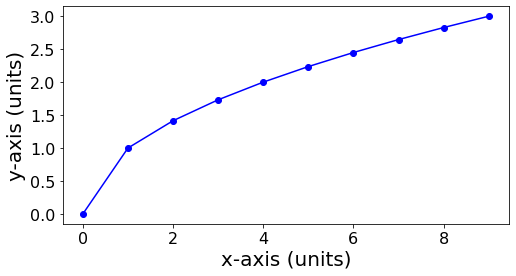
\includegraphics[width=2.5in]{plot.png} 
  \caption{Description with the main take-away point. Note that figure captions should appear below the figure.}
  \label{fig:example} 
\end{figure} 

\subsection{Results on Application/Follow-up Study B} 

\section{Required: Discussion} 

\emph{This is probably the most important section of your paper!  This
  is where you tell us how your work advances our understanding of
  machine learning and healthcare.}  Discuss both technical and
clinical implications, as appropriate.

\paragraph{Limitations}

Explain when your approach may not apply, or things you could not
check.  \emph{Discussing limitations is essential.  Both ACs and
  reviewers have been advised to be skeptical of any work that does
  not consider limitations.}

% ACKNOWLEDGEMENTS ONLY GO IN THE CAMERA-READY, NOT THE SUBMISSION
% \acks{Many thanks to all collaborators and funders!}

\bibliography{sample}

\appendix
\section*{Appendix A.}

Some more details about those methods, so we can actually reproduce
them.  After the blind review period, you could link to a repository
for the code also.  \emph{MLHC values both rigorous evaluation as well
  as reproduciblity.}

\end{document}
